%!TEX TS-program = xelatex
%!TEX engine = xelatex

\documentclass{standalone}

\usepackage{fontspec}
\setmainfont{Fira Mono}
\usepackage{unicode-math}
\setmathfont[Scale=MatchUppercase]{STIX Two Math}
\setmathrm[Scale=MatchUppercase,
           BoldFont=STIX Two Text Bold]{STIX Two Math}
\setmathtt[Scale=MatchUppercase]{Fira Mono}

\usepackage{tikz}

\begin{document}
  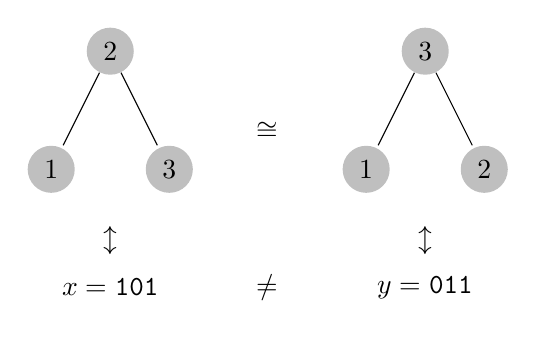
\begin{tikzpicture}[shorten >=1pt]
  \tikzstyle{vertex}=[circle,fill=black!25,minimum size=17pt,inner sep=0pt]

  \node[vertex] (a) {2}
    child {node[vertex] {1}}
    child {node[vertex] {3}};

  \node at (2, -1) {\(\cong\)};

  \node[vertex] at (4, 0) (b) {3}
    child {node[vertex] {1}}
    child {node[vertex] {2}};

  \node at (0, - 2.4) {\(\updownarrow\)};

  \node at (0, - 3) {\(x = \mathtt{101}\)};

  \node at (2, - 3) {\(≠\)};

  \node at (4, - 3) {\(y = \mathtt{011}\)};

  \node at (4, - 2.4) {\(\updownarrow\)};

  \end{tikzpicture}
\end{document}
